\chapter{State Feedback Design}

\section{Principles}

From the state-space model as described by
\begin{align}
\dot{\vec{x}}(t) &= \vec{A} x(t) + \vec{B} u(t) \label{Eq_StSpModel} \\
\vec{y}(t) &= \vec{C} x(t) + \vec{D} u(t)
\end{align}
It was found that the behavior of the system depends on the Eigenvalues of matrix A, which are also the poles of the open-loop system. From the feedback design principles from classical control theory, it was found that the required behavior of a system can be achieved by first closing the loop (getting required output variables) and changing the poles of this closed-loop system so as to match the desired behavior (by changing the dynamics of the system). In state feedback design, a process something similar is used. The idea with control design is to modify the Eigenvalues of system matrix A by using a control input $u(t)$. The difference state-space based feedback design is that contrary to classical design of using system output $y(t)$ for feedback design, here a measured state variable $x(t)$ is used.

The state feedback control design can be expressed mathematically as
\begin{equation}\label{Eq_StSpFBD_ControlEquation}
	u(t) = -Kx(t) + k_r r(t)
\end{equation}
The measured state variable $x(t)$ is used to calculate the desired control action required with a feedback gain $K$ to amplify / attenuate the measured state-variables. Additionally, the error concept similar to classical control design can be implemented using the reference signal $r(t)$ with steady-state reference gain $k_r$ so as to make the system track the desired steady-state.

Equation \eqref{Eq_StSpFBD_ControlEquation} can be read as one control action ($-Kx(t)$) to reduce the dynamics by any input and other control action ($k_r r(t)$) to amplify the system towards the steady-state. Additionally, the control action is negative towards the state gain $-Kx(t)$, that is because, the idea is to reduce the dynamics of the system fo give input, rather than amplify them. In most of the control design approaches the idea of attenuating the dynamics is widely employed.

From the initial design of state feedback system which was essentially an open-loop as shown in figure \ref{Fig_StSp_OL_Design} (here, A is not a feedback matrix, but is instead required to calculate the dynamics $\dot{x}$), the state feedback design is essentially now a feedback with a measured state $x(t)$ as shown in figure \ref{Fig_StSp_CL_Design}. Further, in most of the system, the feed-through matrix D is not used to influence the system output, therefore, in general, the state feedback design of the system is as shown in figure \ref{Fig_StSp_without_D}.
\begin{figure}[h!]
	\centering
	\includegraphics[width=0.6\linewidth]{Bilder/StSp_OL_Design}
	\caption{Block diagram of state-space model}
	\label{Fig_StSp_OL_Design}
\end{figure}
\begin{figure}[h!]
	\centering
	\includegraphics[width=0.6\linewidth]{Bilder/StSp_CL_Design}
	\caption{Block diagram of state feedback model}
	\label{Fig_StSp_CL_Design}
\end{figure}
\begin{figure}[h!]
	\centering
	\includegraphics[width=0.6\linewidth]{Bilder/StSp_without_D}
	\caption{Block diagram of state feedback model without D}
	\label{Fig_StSp_without_D}
\end{figure}
\newpage

Using the control equation now in the state equation, the state equation becomes
\begin{align}
	\dot{\vec{x}}(t) &= \vec{A} x(t) + \vec{B} (-Kx(t) + k_r r(t)) \\
					&= (A - B K) x(t) + B k_r r(t) \label{Eq_StSp_FB_Model}
\end{align}
It can be observed that now the new system matrix is given by $(A - B K)$ matrix instead of matrix A in the previous case. With this new system matrix, the control objective can be stated:
\textbf{\textit{Control objective}}: Choose $K$ such that the closed-loop dynamics $A - BK$ get desired properties such as stability, tracking etc,.

The size of $K$ matrix can be obtained using the relationship $u = - K x$, so if the inputs are of the size $m \times 1$ and the states $x$ are of the size $n \times 1$, then the $K$ matrix should be equal to a size $(m \times n)$ in order to satisfy the relation $u = - K x$.

\subsection{Poles of the closed loop system}

Equation \eqref{Eq_StSp_FB_Model} gives a closed loop (state feedback) system, in order to find the poles, similar to previous open-loop models, a LT is performed on equation \eqref{Eq_StSp_FB_Model}
\begin{equation}
	s X(s) = (A - B K) X(s) + B k_r R(s) \implies (sI - (A - BK))X(s) = B k_r R(s)
\end{equation}
substituting in the LT of the output equation (lets consider matrix D to be a zero matrix)
\begin{equation}
	Y(s) = C X(s) \implies C [(sI - (A - BK))]^{-1} B k_r R(s)
\end{equation}
the TF of the closed-loop system is then
\begin{equation} \label{Eq_StSp_CL_TF}
	G(s) = \frac{Y(s)}{R(s)} = \frac{C B k_r}{sI - (A - BK)}
\end{equation}
The poles of the closed-loop system is given by the values of the denominator of the TF \eqref{Eq_StSp_CL_TF}, which can be found by setting the denominator of TF to zero
\begin{equation} \label{Eq_StSp_CL_Poles}
	\{p\} := det\{sI - (A - BK)\} = 0
\end{equation}

In expressions containing matrices, the expression is set to zero first by taking the determinant which gives the value of the matrix and then setting the value of the determinant to zero.

\subsection{Reference tracking}

The steady-state reference gain $k_r$ does not affect the stability of the system, but it does affect the steady-state solution. And choosing steady-state depends on the tracking required. A $k_r$ is chosen such that
$$	y(t) \approx r(t) \quad t \rightarrow \infty $$
And to choose the steady-state reference gain, the steady-state of the system has to be determined. This can be done by using the state and the output equations and solve them at the steady-state. For a differential $\dot{x}$, the steady-state is when $\dot{x} = 0$
\begin{align}
	0 &= (A - B K) x(t) + B k_r r(t) \\
	y(t) &= C x(t) + D u(t)
\end{align}
Additionally, in most of the system matrix D is zero, therefore
\begin{align}
0 &= (A - B K) x(t) + B k_r r(t) \\
y(t) &= C x(t) \label{Eq_StSp_FBD_Output}
\end{align}
therefore, the steady-state can be expressed by solving the above equation for $x(t)$ and substituting in the output equation
\begin{equation} \label{Eq_StFBD_SS_eq}
	y(t) = -C (A - B K)^{-1} B k_r r(t)
\end{equation}
Finally, using the steady-state output equation, steady-state reference gain $k_r$ can be determined using the condition $y(t) \approx r(t) \quad t \rightarrow \infty$. From equation \eqref{Eq_StFBD_SS_eq},
\begin{equation}
	k_r = (-C (A - B K)^{-1} B)^{-1}
\end{equation}
or
\begin{equation} \label{Eq_StSp_ss_ref_gain_eq}
	k_r = \frac{1}{-C (A - B K)^{-1} B}
\end{equation}

In summary, the design of state feedback is a two step process, first for $K$ and then fro $k_r$.

\section{Integral control}

Although using state-space model by designing a steady-state reference gain $k_r$ to track the reference $r(t)$, in reality due to model inconsistencies (with the real model), the ss will in general not be tracked perfectly by the controller designed using equation \eqref{Eq_StSpFBD_ControlEquation}. In such a case, similar to the classical control design, a integral control action is implemented so as to track the error and apply a control proportional to it. 

In the state-feedback model in equation \eqref{Eq_StSp_FB_Model} there is no variable to track the error, therefore, new state has to be introduced that tracks the error being added up into the system due to ss-error. Suppose the state is introduced as
\begin{equation}
	z(t) = \int (y(t) - r(t)) dt
\end{equation}
the state derivative is then
\begin{equation}
	\dot{z}(t) = y(t) - r(t)
\end{equation}
Now with this additional state along with the original state equation of the system \eqref{Eq_StSpModel}, the two states can be tracked by the model
\begin{equation}
	\begin{bmatrix}
		\dot{x} \\ \dot{z}
	\end{bmatrix} = \begin{bmatrix}
		Ax + Bu \\ y - r
	\end{bmatrix}
\end{equation}
From equation \eqref{Eq_StSp_FBD_Output}, $y = Cx$ using this
\begin{equation}
	\begin{bmatrix}
	\dot{x} \\ \dot{z}
	\end{bmatrix} = \begin{bmatrix}
	Ax + Bu \\ Cx - r
	\end{bmatrix} \implies \begin{bmatrix}
		A & 0 \\ C & 0
	\end{bmatrix} \begin{bmatrix}
	{x} \\ {z}
	\end{bmatrix} + \begin{bmatrix}
		B \\ 0
	\end{bmatrix} u + \begin{bmatrix}
		0 \\ -1
	\end{bmatrix} r
\end{equation}
where the control signal is now given by
\begin{equation}
	u(t) = -Kx(t) - K_I z(t) + k_r r(t)
\end{equation}

\section{Example of State-feedback design} \label{Example_SingleTrackModel}

Consider an example dynamics given of a single track model, where the two states are lateral position and orientation angle respectively.
\begin{align}
	\begin{bmatrix}
		\dot{x}_1 \\ \dot{x}_2
	\end{bmatrix} &= \begin{bmatrix}
		0 & v_0 \\ 0 & 0
	\end{bmatrix} \begin{bmatrix}
	{x}_1 \\ {x}_2
	\end{bmatrix} + \begin{bmatrix}
	a v_0/b \\ v_0 / b
	\end{bmatrix} u \label{Eq_StSp_Ex_DynamicsEq} \\
	y &= [1 \quad 0] \begin{bmatrix}
	{x}_1 \\ {x}_2 \end{bmatrix} + [0] u
\end{align}
with given parameters $v_0 = 12 m/s$, $a = 2$m, $b = 4$m. The input $u$ is the steering angle $\delta$. The idea is to design a controller that stabilizes the dynamics and tracks a given lateral position of the vehicle. This condition is a simplified way of a lane keeping control.

Starting from the controller equation, we have two states $x_1$ and $x_2$
\begin{equation} \label{Eq_StSp_CL_ControlEq}
	u(t) = -Kx(t) + k_r r(t) = u = -K_{1}x_{1} - K_{2}x_{2} + k_r r
\end{equation}
The closed loop system dynamics are obtained by using the closed-loop control equation \eqref{Eq_StSp_CL_ControlEq} to the state equation \eqref{Eq_StSp_Ex_DynamicsEq}
\begin{equation}
	\dot{x} = (A - B K) x(t) + B k_r r(t) \implies \dot{x} = (A - [B] [K_1 \quad K_2]) x(t) + B k_r r(t)
\end{equation}
\begin{equation}
	\begin{bmatrix}
	\dot{x}_1 \\ \dot{x}_2
	\end{bmatrix} = \left( \begin{bmatrix}
	0 & v_0 \\ 0 & 0
	\end{bmatrix} - \begin{bmatrix}
	a v_0/b \\ v_0 / b
	\end{bmatrix} [K_1 \quad K_2] \right) \begin{bmatrix}
	{x}_1 \\ {x}_2
	\end{bmatrix} + \begin{bmatrix}
	a v_0/b \\ v_0 / b
	\end{bmatrix} k_r r
\end{equation}
\begin{equation}
	\begin{bmatrix}
	\dot{x}_1 \\ \dot{x}_2
	\end{bmatrix} = \begin{bmatrix}
	-K_{1} a v_{0}/b & v_0 -K_{2} a v_{0}/b \\ -K_{1} v_{0}/b & -K_{2} v_{0}/b
	\end{bmatrix} \begin{bmatrix}
	{x}_1 \\ {x}_2
	\end{bmatrix} + \begin{bmatrix}
	k_{r} a v_0/b \\ k_{r} v_0 / b
	\end{bmatrix} r
\end{equation}
The closed-loop poles are determined using equation \eqref{Eq_StSp_CL_Poles} for state feedback controller. In order to design the parameters of the controller, a pole-placement technique is used similar to classical control design. Therefore, choosing a desired polynomial to do so as
\begin{equation}
	\lambda^{2} + 2 \zeta \omega_{n} \lambda + \omega_{n}^{2}
\end{equation}
using equation \eqref{Eq_StSp_CL_Poles}, the characteristic equation for this example problem can be found as
\begin{equation}
	det(\lambda I - A + BK) = \lambda^{2} + \frac{v_0}{b} (aK_{1} + K_{2}) \lambda + \frac{K_{1} v_{0}^{2}}{b}
\end{equation}
matching coefficients with desired polynomial
\begin{equation}
	\lambda^{2} + 2 \zeta \omega_{n} \lambda + \omega_{n}^{2} = \lambda^{2} + \frac{v_0}{b} (aK_{1} + K_{2}) \lambda + \frac{K_{1} v_{0}^{2}}{b}
\end{equation}
the feedback gain can be determined as
\begin{align}
	K_1 &= \frac{b \omega_{n}^{2}}{v_{0}^{2}} \\
	K_2 &= \frac{2 \zeta \omega_{n} b}{v_0} - \frac{a b \omega_{n}^{2}}{v_{0}^{2}}
\end{align}
A feedback gain in the system stabilizes the system through pole placements. However, for tracking, the system also should now track the reference $r(t)$ for which the ss-reference gain $k_r$ should be designed. This $k_r$ value can be determined using the previously determined equation for $k_r$ equation \eqref{Eq_StSp_ss_ref_gain_eq}
\begin{equation}
	k_r = \frac{1}{-C (A - B K)^{-1} B} \implies k_r = \frac{b \omega_{n}^{2}}{v_{0}^{2}}
\end{equation}
therefore, now the controller equation becomes
\begin{equation}
	u = -K_{1}x_{1} - K_{2}x_{2} + k_r r \implies = -\frac{b \omega_{n}^{2}}{v_{0}^{2}} x_{1} - \frac{2 \zeta \omega_{n} b}{v_0} - \frac{a b \omega_{n}^{2}}{v_{0}^{2}} x_{2} + \frac{b \omega_{n}^{2}}{v_{0}^{2}} r
\end{equation}

Further, the behavior of this closed loop system can be determined by using simulations, simulating for different values to system parameters $\zeta$ and $\omega_{n}$. For a unit step input, the following results can be visualized in Simulink as shown in figure \ref{Fig_StSp_FD_Ex1}
\begin{figure}[h!]
	\centering
	\includegraphics[width=\linewidth]{Bilder/StSp_FD_Ex1}
	\caption{Simulation results for different design parameters}
	\label{Fig_StSp_FD_Ex1}
\end{figure}
Running another simulation for a trajectory which is sinusoidal and see if the model is tracking the reference signal. For such a purpose a sinusoidal trajectory was chosen such that it produces an oscillation of $2 \pi$ time period $10$s. Figure \ref{Fig_StSp_FD_Ex1_1} shows the tracking of the system for the reference input.
\begin{figure}[h!]
	\centering
	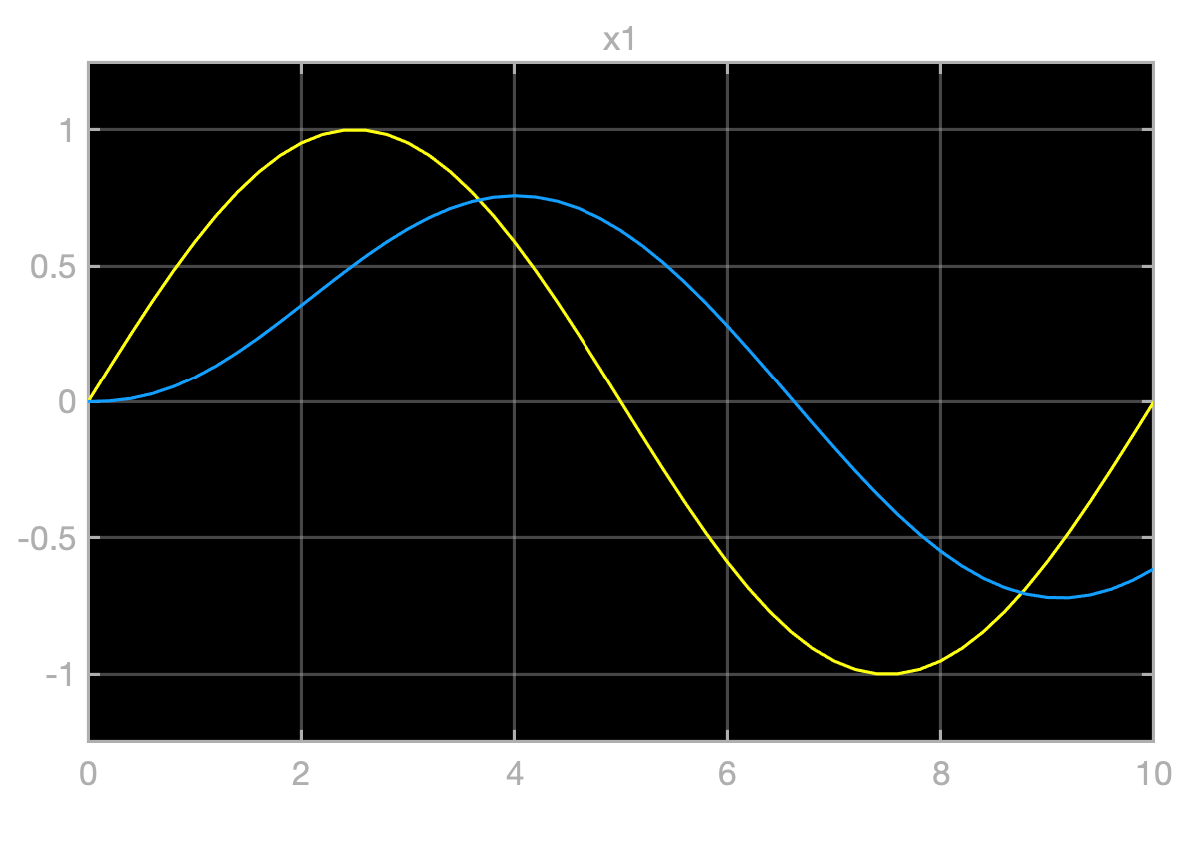
\includegraphics[width=0.65\linewidth]{Bilder/StSp_FD_Ex1_1.eps}
	\caption{Simulation results for sinusoidal trajectory}
	\label{Fig_StSp_FD_Ex1_1}
\end{figure}
\newpage
It can be seen from figure \ref{Fig_StSp_FD_Ex1_1} that the system is able to trace the trajectory by the raise time is too big. From figure \ref{Fig_StSp_FD_Ex1} for the simulations for a step-response, it can be seen that the raise time can be reduced by increasing $\omega_{n}$, therefore setting a larger $\omega_{n}$, the resulting figure is shown in \ref{Fig_StSp_FD_Ex1_2}, reaching a perfect tracking.
\begin{figure}[h!]
	\centering
	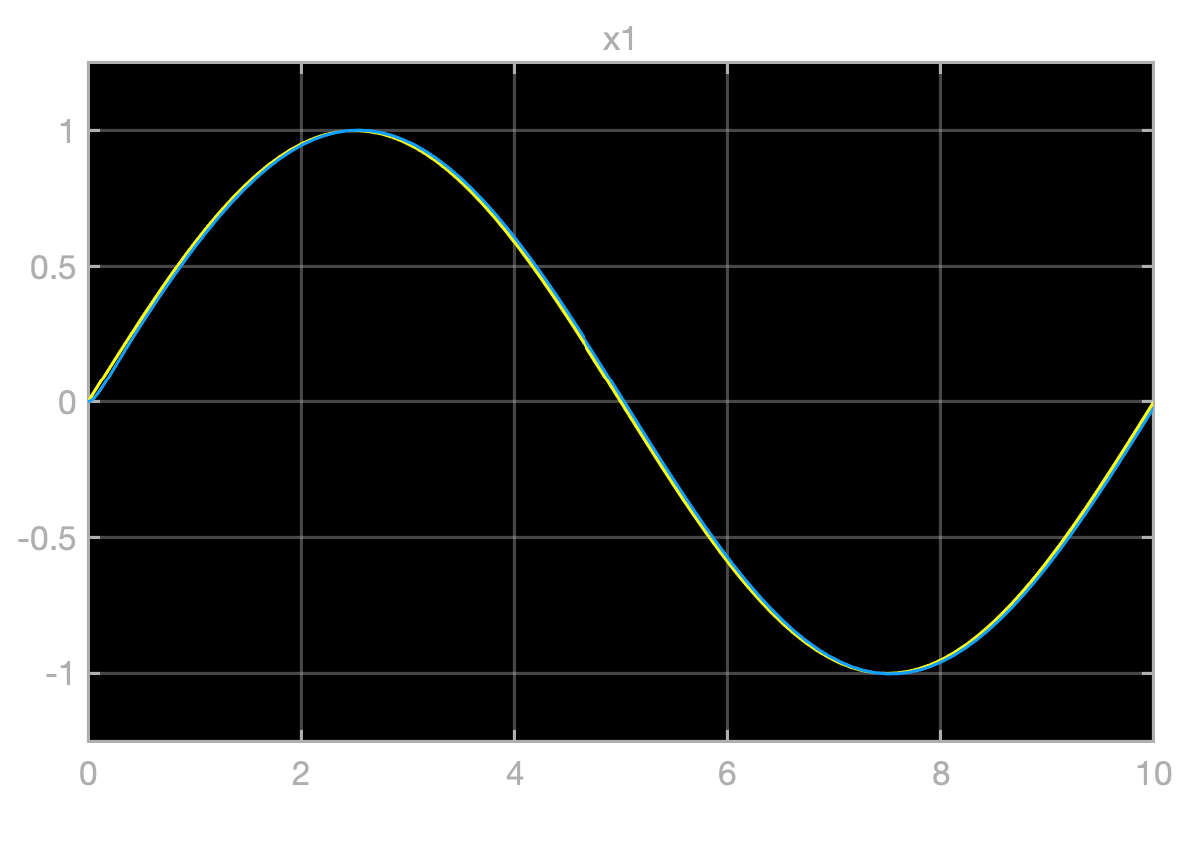
\includegraphics[width=0.65\linewidth]{Bilder/StSp_FD_Ex1_2.eps}
	\caption{Simulation results for sinusoidal trajectory with better tracking}
	\label{Fig_StSp_FD_Ex1_2}
\end{figure}

\section{Example of reaching non-controllability}

Consider another system which is similar to Example 1 but with a different matrix B as given by
\begin{align}
\begin{bmatrix}
\dot{x}_1 \\ \dot{x}_2
\end{bmatrix} &= \begin{bmatrix}
0 & v_0 \\ 0 & 0
\end{bmatrix} \begin{bmatrix}
{x}_1 \\ {x}_2
\end{bmatrix} + \begin{bmatrix}
1 \\ 0
\end{bmatrix} u  \\
y &= [1 \quad 0] \begin{bmatrix}
{x}_1 \\ {x}_2 \end{bmatrix} + [0] u
\end{align}
with control signal same as the previous example
\begin{equation}
u(t) = -Kx(t) + k_r r(t) = u = -K_{1}x_{1} - K_{2}x_{2} + k_r r
\end{equation}
Solving for state dynamics
\begin{align}
	\dot{x} &= (A - BK)x + Bk_r r = \begin{bmatrix}
	-K_{1} & 1-K_{2} \\ 0 & 0
	\end{bmatrix} x + \begin{bmatrix}
	k_{r} \\ 0
	\end{bmatrix} r \\
	 y &= [1 \quad 0] \begin{bmatrix}
	 {x}_1 \\ {x}_2 \end{bmatrix}
\end{align}
Solving for closed-loop system poles
\begin{equation}
	det(\lambda I - A + BK) = det \begin{Bmatrix}
		\lambda + K_{1} & K_{2} - 1 \\ 0 & \lambda
	\end{Bmatrix} = \lambda^{2} + K_{1}\lambda = \lambda (\lambda + K_{1})
\end{equation}
while matching the systems characteristic polynomial, the following two results are observed
\begin{equation}
	\lambda^{2} + 2 \zeta \omega_{n} \lambda + \omega_{n}^{2} = \lambda (\lambda + K_{1})
\end{equation}
\begin{enumerate}
	\item Not all coefficients of characteristic polynomial can be matched with the desired polynomial. That means all the Eigenvalues cannot be controlled. Therefore, the dynamics of the system cannot be shaped. Such a system is not controllable or not reachable.
	\item One of the Eigenvalues is zero, the system is not asymptotically stable (it may oscillate with same magnitude without amplification, such a condition is also not asymptotically stable).
\end{enumerate}